% \begin{figure}[h!]
%     \begin{subfigure}{.5\textwidth}
%     \centering
%     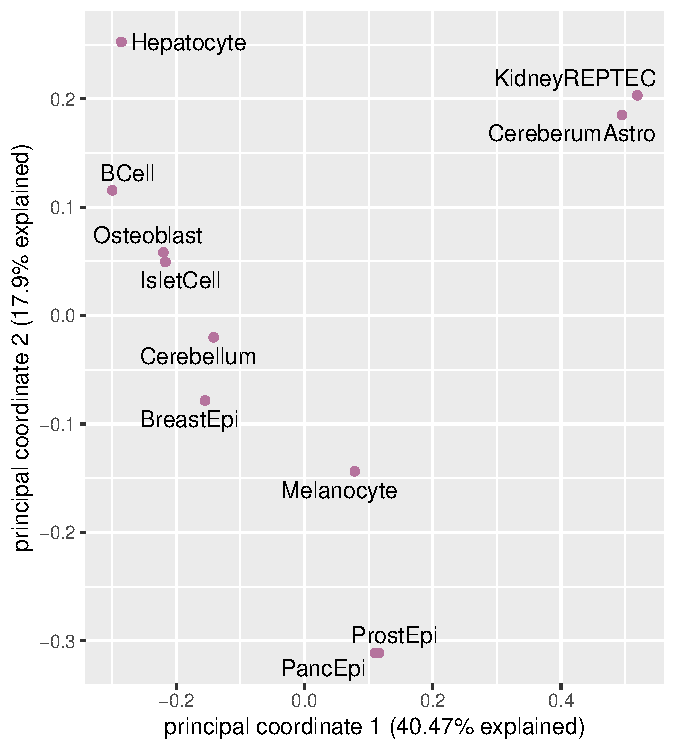
\includegraphics[scale=0.7]{graphics/encode_pca_1_2.pdf}
%     \caption{PC2 \textit{v.s.} PC1}
%     \end{subfigure}
%     ~
%     \begin{subfigure}{.5\textwidth}
%     \centering
%     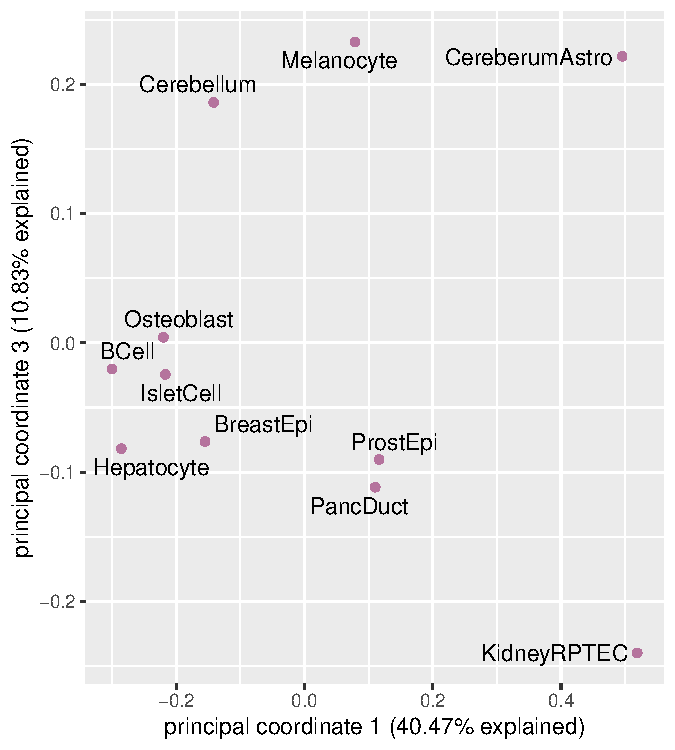
\includegraphics[scale=0.7]{graphics/encode_pca_1_3.pdf}
%     \caption{PC3 \textit{v.s.} PC1}
%     \end{subfigure} \\
%     \caption{\textbf{PCA}.}
%     \label{fig:encode_pca}
% \end{figure}

\begin{figure}[h!]
  \begin{minipage}[c]{\textwidth}
    \begin{subfigure}{.5\textwidth}
    \centering
    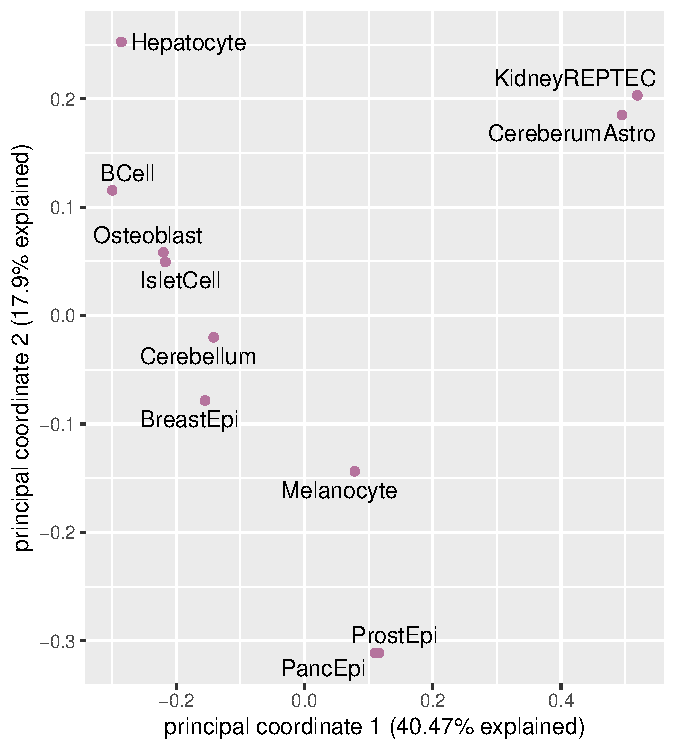
\includegraphics[scale=0.7]{graphics/encode_pca_1_2.pdf}
    \caption{PC2 \textit{v.s.} PC1}
    \end{subfigure}
    ~
    \begin{subfigure}{.5\textwidth}
    \centering
    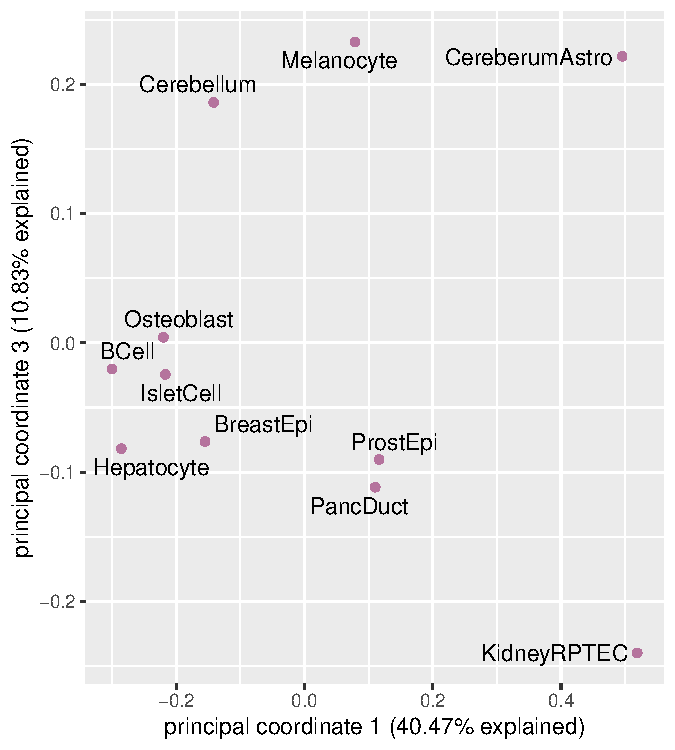
\includegraphics[scale=0.7]{graphics/encode_pca_1_3.pdf}
    \caption{PC3 \textit{v.s.} PC1}
    \end{subfigure} \\
  \end{minipage}\hfill
  \vspace{1cm}
  
  \begin{minipage}[c]{\textwidth}
    \centering
    \begin{tabulary}{\textwidth}{ ll }
    \toprule
    \textbf{Original cell abbreviation} & \bf{Cancer Type}  \\
    \toprule
    Osteoblast & Osteosarcoma \\
    
    BreastEpi & Breast-AdenoCa \\
    
    Cerebellum &  CNS-Medullo  \\
    
    CereberumAstro & CNS-PiloAstro \\
    
    KidneyRPTEC & Kidney-RCC \\
    
    Hepatocyte & Liver-HCC \\
    
    BCell & Lymph-BNHL, Lymph-CLL \\
    
    PancDuct & Panc-AdenoCa \\
    
    IsletCell & Panc-Endocrine \\
    
    ProstEpi & Prost-AdenoCa \\
    
    Melanocyte & Skin-Melanoma \\
    \bottomrule
    
    \end{tabulary}
    
    % . DHS data for these cells is downloaded from either \href{https://genome.ucsc.edu/cgi-bin/hgFileUi?db=hg19&g=wgEncodeOpenChromDnase}{Duke} or \href{https://genome.ucsc.edu/cgi-bin/hgFileUi?db=hg19&g=wgEncodeUwDnase}{UW} project
  \end{minipage}\hfill
  \vspace{0.9cm}
  
  \begin{minipage}[c]{\textwidth}
    \caption{
    %   \textbf{Some cancers were more related in terms of chromatin structures than others.} Here, I visualised the relative coordinates of the original cell types for cancers on the most informative dimensions (principle coordinates, PC). The informativeness of each PC manifests in the percentage of variance explained. This was done by multidimensional scaling of the pairwise distance between cell types. The distance between two cell types was computed based on the intersection between their open chromatin regions. 
    } \label{fig:encode_pca}
  \end{minipage}
\end{figure}
